
The general equation of circle can be expressed as
\begin{align}
    \vec{x}^T\vec{x}-2\vec{c}^T\vec{x}+f = 0\label{eq:solutions/4/1/1/a/eq:1}
\end{align}
where $\vec{c}$ is the centre of the circle and radius of the circle is given as
\begin{align}
r = \sqrt{\norm{\vec{c}}^2 - f}\label{eq:solutions/4/1/1/a/eq:2}
\end{align}
Given equation is
\begin{align}
3\vec{x}^T\vec{x}+\myvec{-12 & 6}\vec{x}+ 11 = 0\\
\vec{x}^T\vec{x}+\myvec{-4 & 2}\vec{x}+ \frac{11}{3} = 0\\
\vec{x}^T\vec{x}-2\myvec{2 & -1}\vec{x}+ \frac{11}{3} = 0\label{eq:solutions/4/1/1/a/eq:3}
\end{align}
Compare Eq \eqref{eq:solutions/4/1/1/a/eq:1} and Eq \eqref{eq:solutions/4/1/1/a/eq:3}
\begin{align}
\implies\vec{c}^{T} = \myvec{2 & -1}\\
\implies\vec{c} = \myvec{2 \\ -1}\label{eq:solutions/4/1/1/a/eq:4}\\
f = \frac{11}{3}
\end{align}
From Eq \eqref{eq:solutions/4/1/1/a/eq:2},
\begin{align}
    \implies r=\sqrt{\brak{2^2 + \brak{-1}^2} - \frac{11}{3}}\\
    = \sqrt{4 + 1 - \frac{11}{3}}\\
    = \sqrt{\frac{4}{3}}\label{eq:solutions/4/1/1/a/eq:5}
\end{align}
From Eq \eqref{eq:solutions/4/1/1/a/eq:4} and Eq \eqref{eq:solutions/4/1/1/a/eq:5}
\begin{align}
   \vec{c} = \myvec{2 \\ -1}\\
    r = \sqrt{\frac{4}{3}}
\end{align}
\begin{figure}[!ht]
\centering
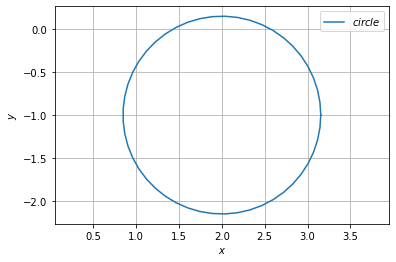
\includegraphics[width=\columnwidth]{./solutions/4/1/1/a/A4.png}
\caption{Circle with radius 1.154 and center coordinates (2,-1)}
\label{eq:solutions/4/1/1/a/Fig:1}
\end{figure}
